\section{Methodology}

In this section, we first outline the model architecture, then the manually crafted features, and finally how they are  incorporated into the model.

\subsection{Model Architecture}
\begin{figure}[tb]
\centering
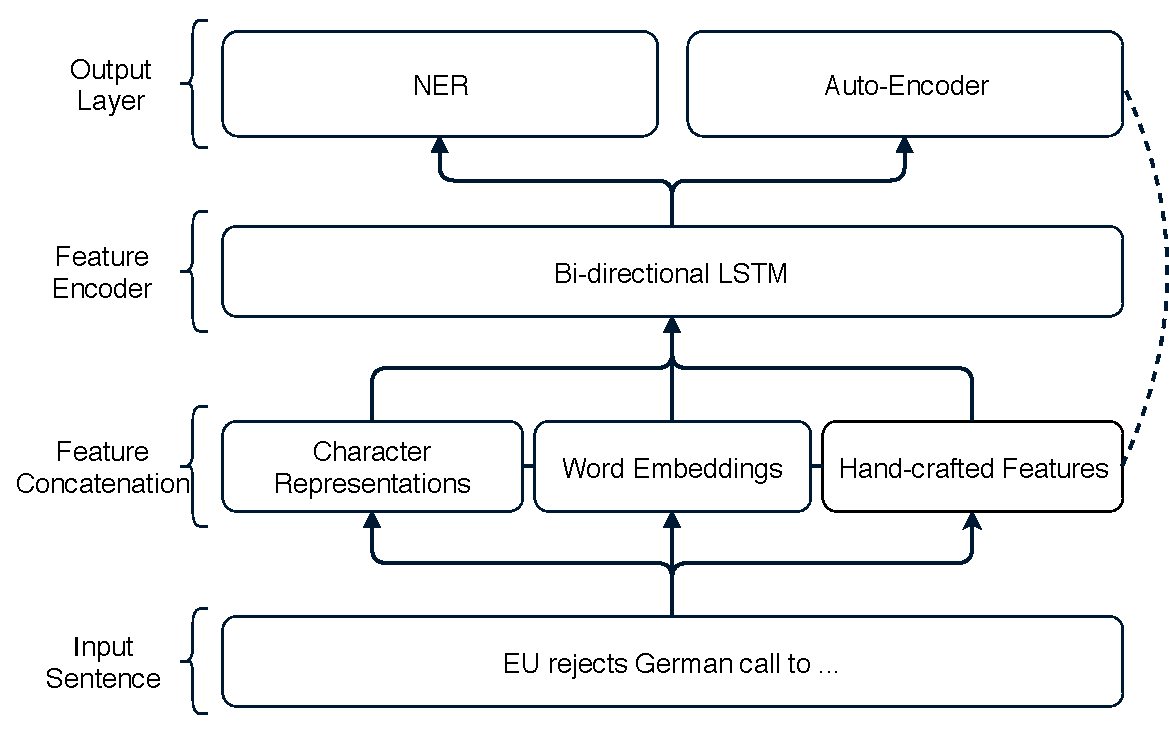
\includegraphics[width=\columnwidth]{model}
\caption{Main architecture of our neural network. Character representations are extracted by a character-level CNN. The dash line indicates we use an auto-encoder loss to reconstruct hand-crafted features.}
\label{figure1}
\end{figure}

We build on a highly competitive sequence labelling model, namely Bi-LSTM-CNN-CRF, first introduced by \newcite{ma2016end}. 
Given an input sequence of $\mathbf{x} = \{x_{1}, x_2, \ldots, x_T\}$ of length $T$, the model is capable of tagging each input with a predicted label $\hat{y}$, resulting in a sequence of $\hat{\mathbf{y}} = \{\hat{y}_1, \hat{y}_2, \ldots, \hat{y}_T\}$ closely matching the gold label sequence $\mathbf{y} = \{y_1, y_2, \ldots, y_T\}$. 
Here, we extend the model by incorporating an auto-encoder loss taking hand-crafted features as in/output, thereby forcing the model to preserve crucial information stored in such features and allowing us to evaluate the impacts of each feature on model performance. 
Specifically, our model, referred to as Neural-CRF+AE, consists of four major components: (1) a character-level CNN (char-CNN); (2) a word-level bi-directional LSTM (Bi-LSTM); (3) a conditional random field (CRF); and (4) an auto-encoder auxiliary loss. 
An illustration of the model architecture is presented in \figref{figure1}.

\begin{table*}[!t]
\centering
\small
\begin{tabular}{llllllll}
\toprule
$\mathbf{x}$           & \em U.N.     & \em official & \em  Ekeus    & \em heads & \em for  & \em Baghdad & \em .     \\ 
\midrule
POS        & NNP      & NN       & NNP      & VBZ   & IN   & NNP     & .     \\ 
Word shape      & X.X.     & xxxx     & Xxxxx    & xxxx  & xxx  & Xxxxx   & .     \\ 
Dependency tags & compound & compound & compound & ROOT  & prep & pobj    & punct \\ 
Gazetteer       & O        & O        & PER      & O     & O    & LOC     & O     \\
\midrule
$\mathbf{y}$          & B-ORG      & O        & B-PER      & O     & O    & B-LOC     & O     \\ 
\bottomrule
\end{tabular}
\caption{Example sentence (top), showing the different types of linguistic features used in this work as additional inputs and auxiliary outputs (middle), and its labelling (bottom).}
\label{feature}
\end{table*}

\paragraph{Char-CNN.} 
Previous studies \cite{santos2014learning, chiu2016named, ma2016end} have demonstrated that CNNs are highly capable of capturing character-level features. 
Here, our character-level CNN is similar to that used in \newcite{ma2016end} but differs in that we use a ReLU activation \cite{nair2010rectified}.\footnote{While the hyperbolic tangent activation function results in comparable performance, the choice of ReLU is mainly due to faster convergence.} 

\paragraph{Bi-LSTM.} 
We use a Bi-LSTM to learn contextual information of a sequence of words. 
As inputs to the Bi-LSTM, we first concatenate the pre-trained embedding of each word $\vec[i]{w}$ with its character-level representation $\vec[w_i]{c}$ (the output of the char-CNN) and a vector of manually crafted features $\vec[i]{f}$ (described in \secref{sec:features}): 
\begin{align}
\vecfwd[i]{h} &= \lstmfwd(\vecfwd[i-1]{h}, [\vec[i]{w};\vec[w_i]{c};\vec[i]{f}])\\
\vecbwd[i]{h} &= \lstmbwd(\vecbwd[i+1]{h}, [\vec[i]{w};\vec[w_i]{c};\vec[i]{f}])\,,
\end{align}
where $[;]$ denotes concatenation.
The outputs of the forward and backward pass of the Bi-LSTM is then concatenated $\vec[i]{h} = [\vecfwd[i]{h};\vecbwd[i]{h}]$ to form the output of the Bi-LSTM, where dropout is also applied.

\paragraph{CRF.} 
For sequence labelling tasks, it is intuitive and beneficial to utilise information carried between neighbouring labels to predict the best sequence of labels for a given sentence. 
Therefore, we employ a conditional random field layer \cite{lafferty2001conditional} taking as input the output of the Bi-LSTM $\vec[i]{h}$. 
Training is carried out by maximising the log probability of the gold sequence: $\mathcal{L}_{CRF} = \log p(\mathbf{y}|\mathbf{x})$ while decoding can be efficiently performed with the Viterbi algorithm.

\paragraph{Auto-encoder loss.} 
Alongside sequence labelling as the primary task, we also deploy, as auxiliary tasks, three auto-encoders for reconstructing the hand-engineered feature vectors. 
To this end, we add multiple independent fully-connected dense layers, all taking as input the Bi-LSTM output $\vec[i]{h}$ with each responsible for reconstructing a particular type of feature: $\hat{\vec[i]{f}^{t}} = \sigma(\mat{W}^{t}\vec[i]{h})$ where $\sigma$ is the sigmoid activation function, $t$ denotes the type of feature, and $\mat{W}^{t}$ is a trainable parameter matrix. 
More formally, we define the auto-encoder loss as:
\begin{equation}
\mathcal{L}_{AE}^{t} = \sum_{i=0}^{T}\xentropy(\vec[i]{f}^{t}, \hat{\vec[i]{f}^{t}})\,.
\end{equation}

\myparagraph{Model training.}
Training is carried out by optimising the joint loss:
\begin{equation}
\mathcal{L} = \mathcal{L}_{CRF} + \sum_{t}\lambda^{t}\mathcal{L}_{AE}^{t}\,,
\end{equation}
where, in addition to $\mathcal{L}_{CRF}$, we also add the auto-encoder loss, weighted by $\lambda^t$. In all our experiments, we set $\lambda^t$ to $1$ for all $t$s.

\subsection{Hand-crafted Features}
\label{sec:features}

We consider three categories of widely used features: (1) POS tags; (2) word shape; and (3) gazetteers and present an example in \tabref{feature}.
While POS tags carry syntactic information regarding sentence structure, the word shape feature focuses on a more fine-grained level, encoding character-level knowledge to complement the loss of information caused by embedding lookup, such as capitalisation. 
Both features are based on the implementation of spaCy.\footnote{\url{https://spacy.io/}}
For the gazetteer feature, we focus on \textit{PERSON} and \textit{LOCATION} and compile a list for each. 
The \textit{PERSON} gazetteer is collected from U.S.\ census 2000, U.S.\ census 2010 and DBpedia whereas GeoNames is the main source for \textit{LOCATION}, taking in both official and alternative names. 
All the tokens on both lists are then filtered to exclude frequently occurring common words.\footnote{Gazetteer data is included in the code release.}
Each category is converted into a one-hot sparse feature vector $\vec[i]{f}^{t}$ and then concatenated to form a multi-hot vector $\vec[i]{f} = [\vec[i]{f}^{\textrm{POS}};\vec[i]{f}^{\textrm{shape}};\vec[i]{f}^{\textrm{gazetteer}}]$ for the $i$-th word. 
In addition, we also experimented with including the label of the incoming dependency edge to each word as a feature, but observed performance deterioration on the development set.
While we still study and analyse the impacts of this feature in \tabref{table4} and \secref{ssec:ablation}, it is excluded from our model configuration (not considered as part of $\vec[i]{f}$ unless indicated otherwise).
